In this chapter the final test will be processed, through this chapter, the approach from the test report for the final test will be commented. The test report can be seen in appendix \ref{ap:final_test_report}.


As discussed in section \ref{sec:control_code}, the drone had to be manually flown to the point where it hovers. Here the pilot flips a switch to set the gravity offset thrust, and set the initial set-point. If the operator flips the switch to the next position, 100 mm is added to the set point. Apart from the code explained in section \ref{sec:control_code} there were added a piece of code to track the demanded throttle every 20 ms. Once the aforementioned switch was returned to its initial position, the system would log the last 20 seconds of sampled throttle data to EEPROM on the micro-controller. This data was used in the data processing to compare to the data from the Vicon system.

In the first part of the test, the K$_\text{p}$ is set to the calculated 0.01, from section \ref{sec:design_controller}. The result from this test can be seen on figure \ref{fig:first_test_report}.

\begin{figure}[H]
    \centering
    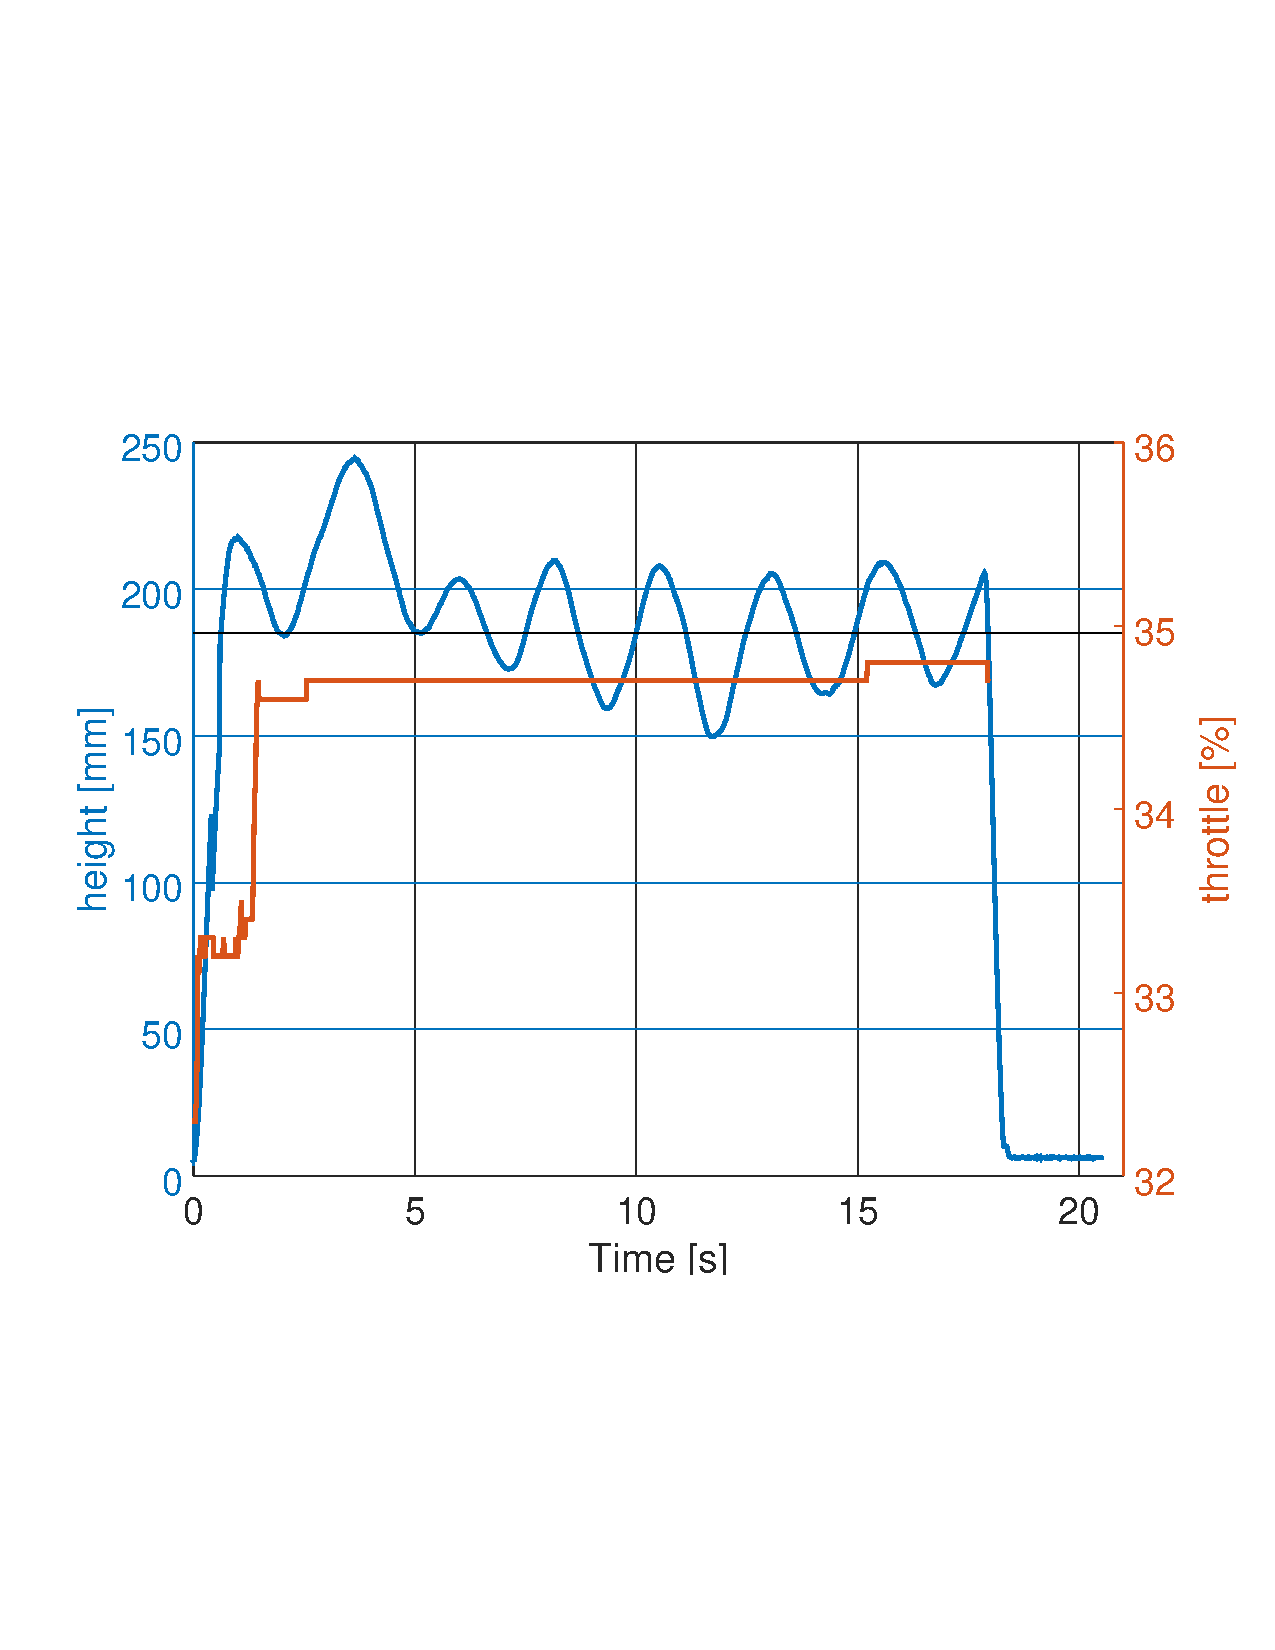
\includegraphics[width=0.6\textwidth, trim={0 7cm 0 7cm},clip]{figures/Appendix/final_test/kp0,012.pdf}
    \caption{Height graph K$_\text{p}$ = 0.01. Marker line is at 185 mm}
    \label{fig:first_test_report}
\end{figure}

From this first test, it was clear the gain was too low. This can be seen by the throttle present only swing with 0.1\% throttle over the gravity offset, on figure \ref{fig:first_test_report}. This is not enough when it is set to make a addition of 100 mm to the height. To compensate for this the K$_\text{p}$ value was set to 0.05, and the test was retried. The result of this test can be seen on figure \ref{fig:second_test_report}.
By making this change to the K$_\text{p}$, the result still did not match the wished result. 
But the result still showed that there were some sort of changing in the throttle present, but still not enough to make the drone raise 100 mm in the height. 
\begin{figure}[H]
    \centering
    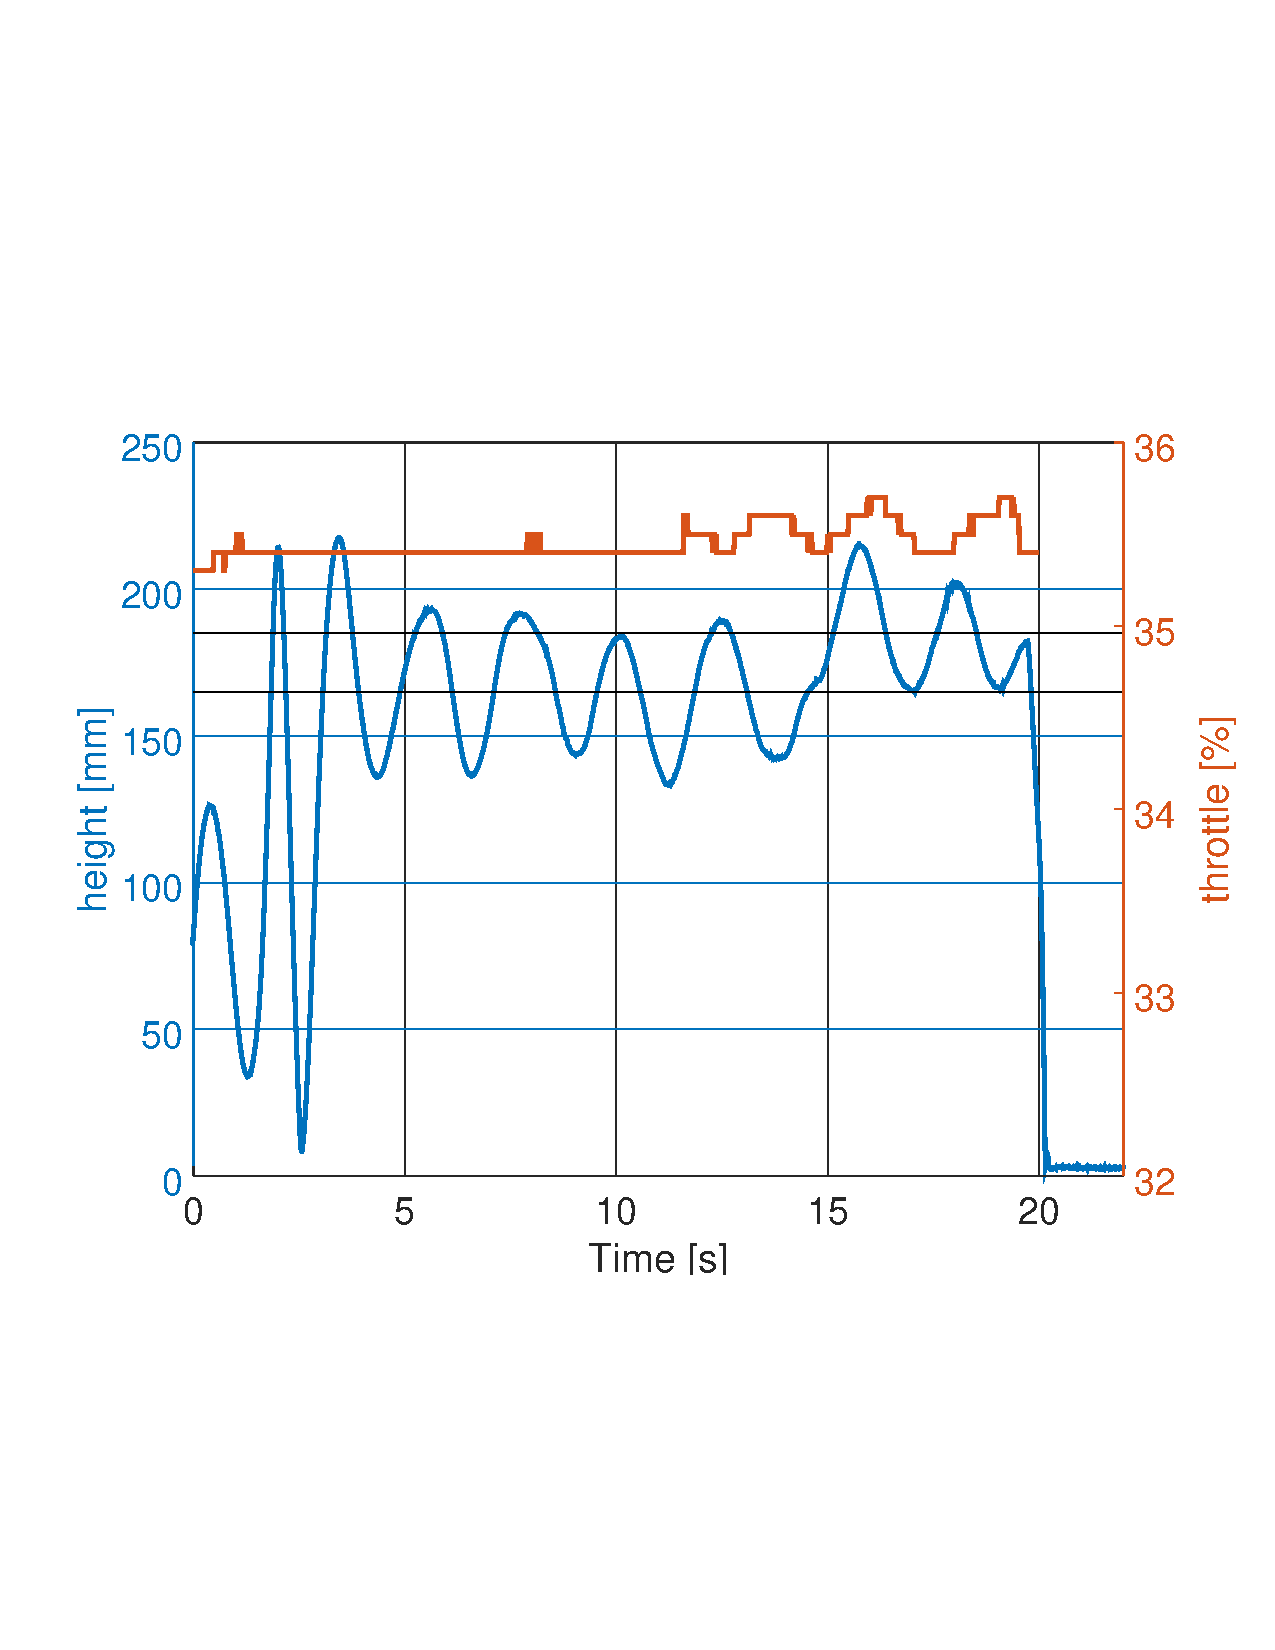
\includegraphics[width=0.6\textwidth, trim={0 7cm 0 7cm},clip]{figures/Appendix/final_test/kp0,05.pdf}
    \caption{Height graph K$_\text{p}$ = 0.05. Marker lines are at 165 and 185 mm}
    \label{fig:second_test_report}
\end{figure}
The K$_\text{p}$ value was further increased, but this gave problems with oscillation, when the K$_\text{p}$ value were set to 0.1, as it can be seen on figure \ref{fig:third_test_report}.
\begin{figure}[H]
    \centering
    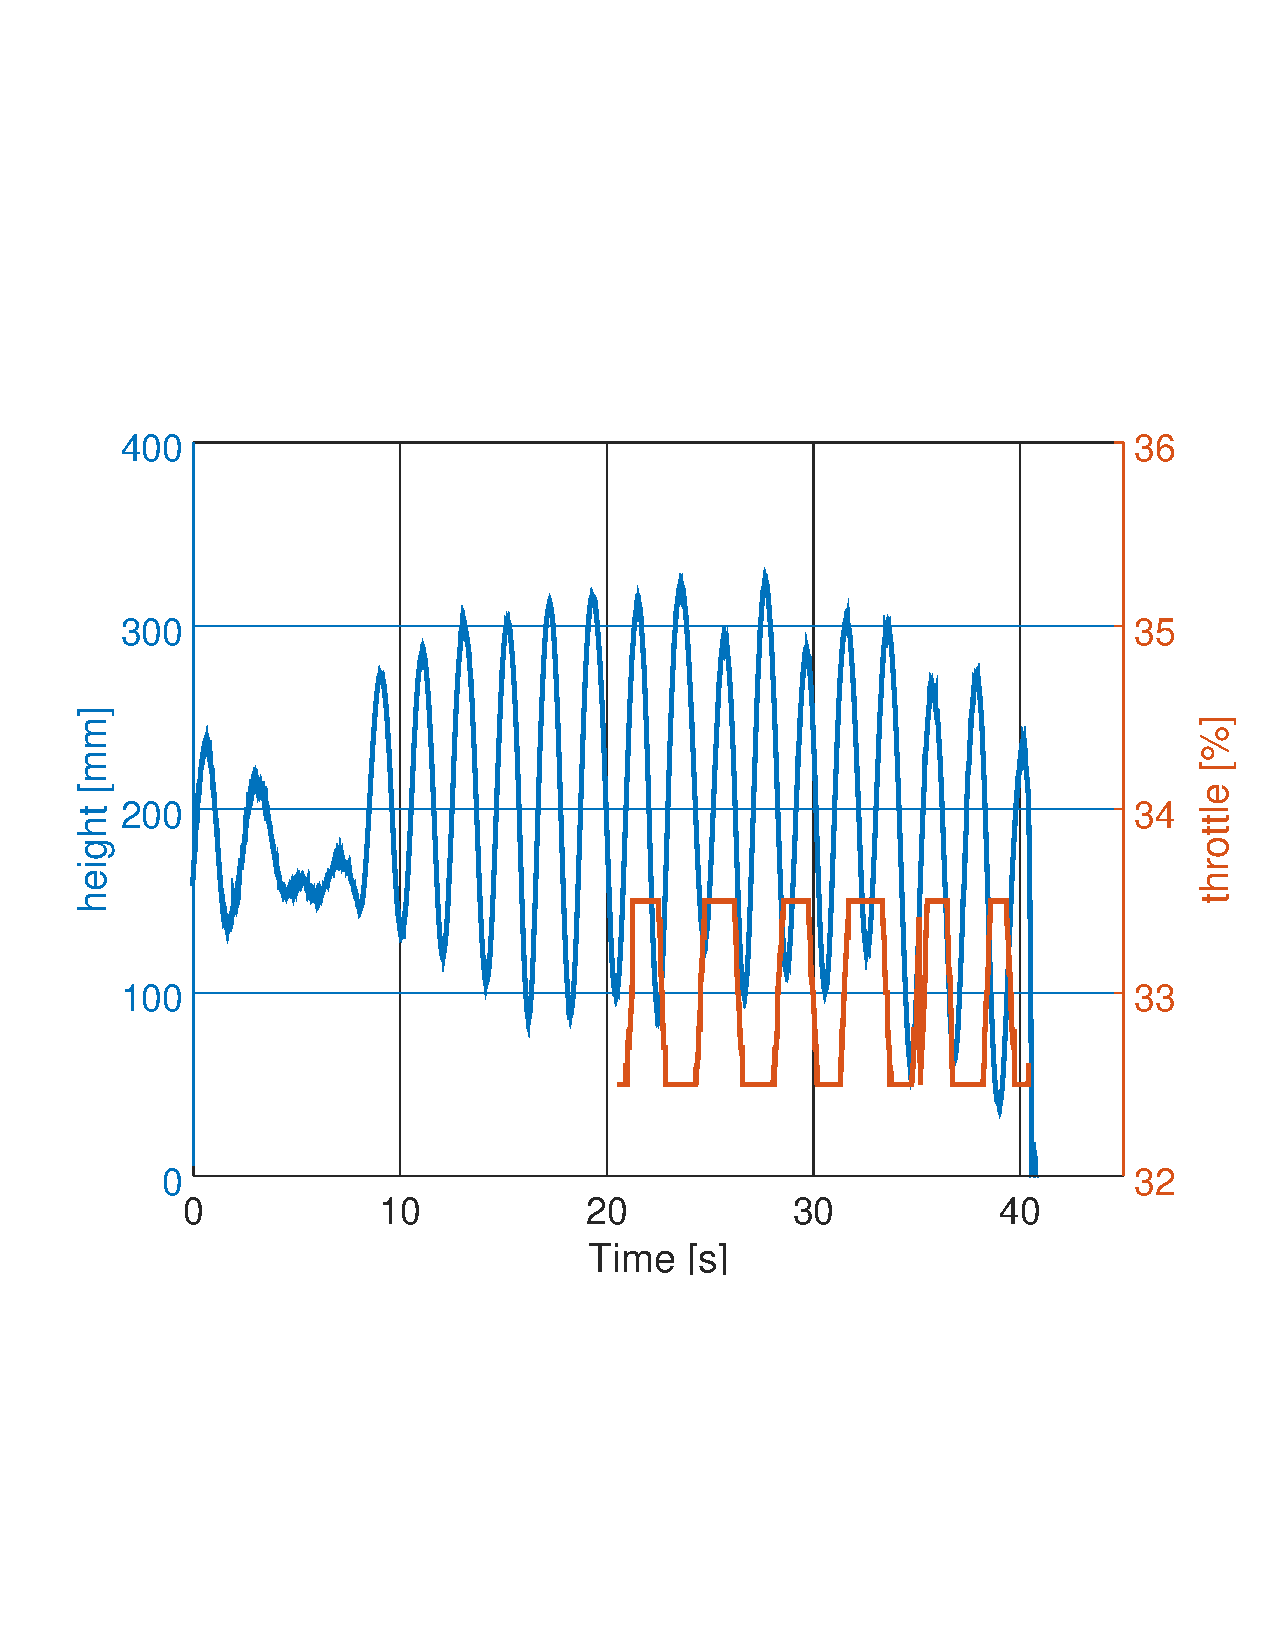
\includegraphics[width=0.6\textwidth, trim={0 7cm 0 7cm},clip]{figures/Appendix/final_test/kp0,1.pdf}
    \caption{Height graph K$_\text{p}$ = 0.1.}
    \label{fig:third_test_report}
\end{figure}

This change in K$_\text{P}$ also highlighted a new issue. In the code, the output throttle was supposed to be limited to 10\% above the offset, which can be seen on figure \ref{fig:third_test_report} the throttle clipped at 1\% swing. This was a simple bug in the code, and once fixed, the results were a bit different. The results without the error in the code can be seen on figure \ref{fig:fourth_test_report}.

\begin{figure}[H]
    \centering
    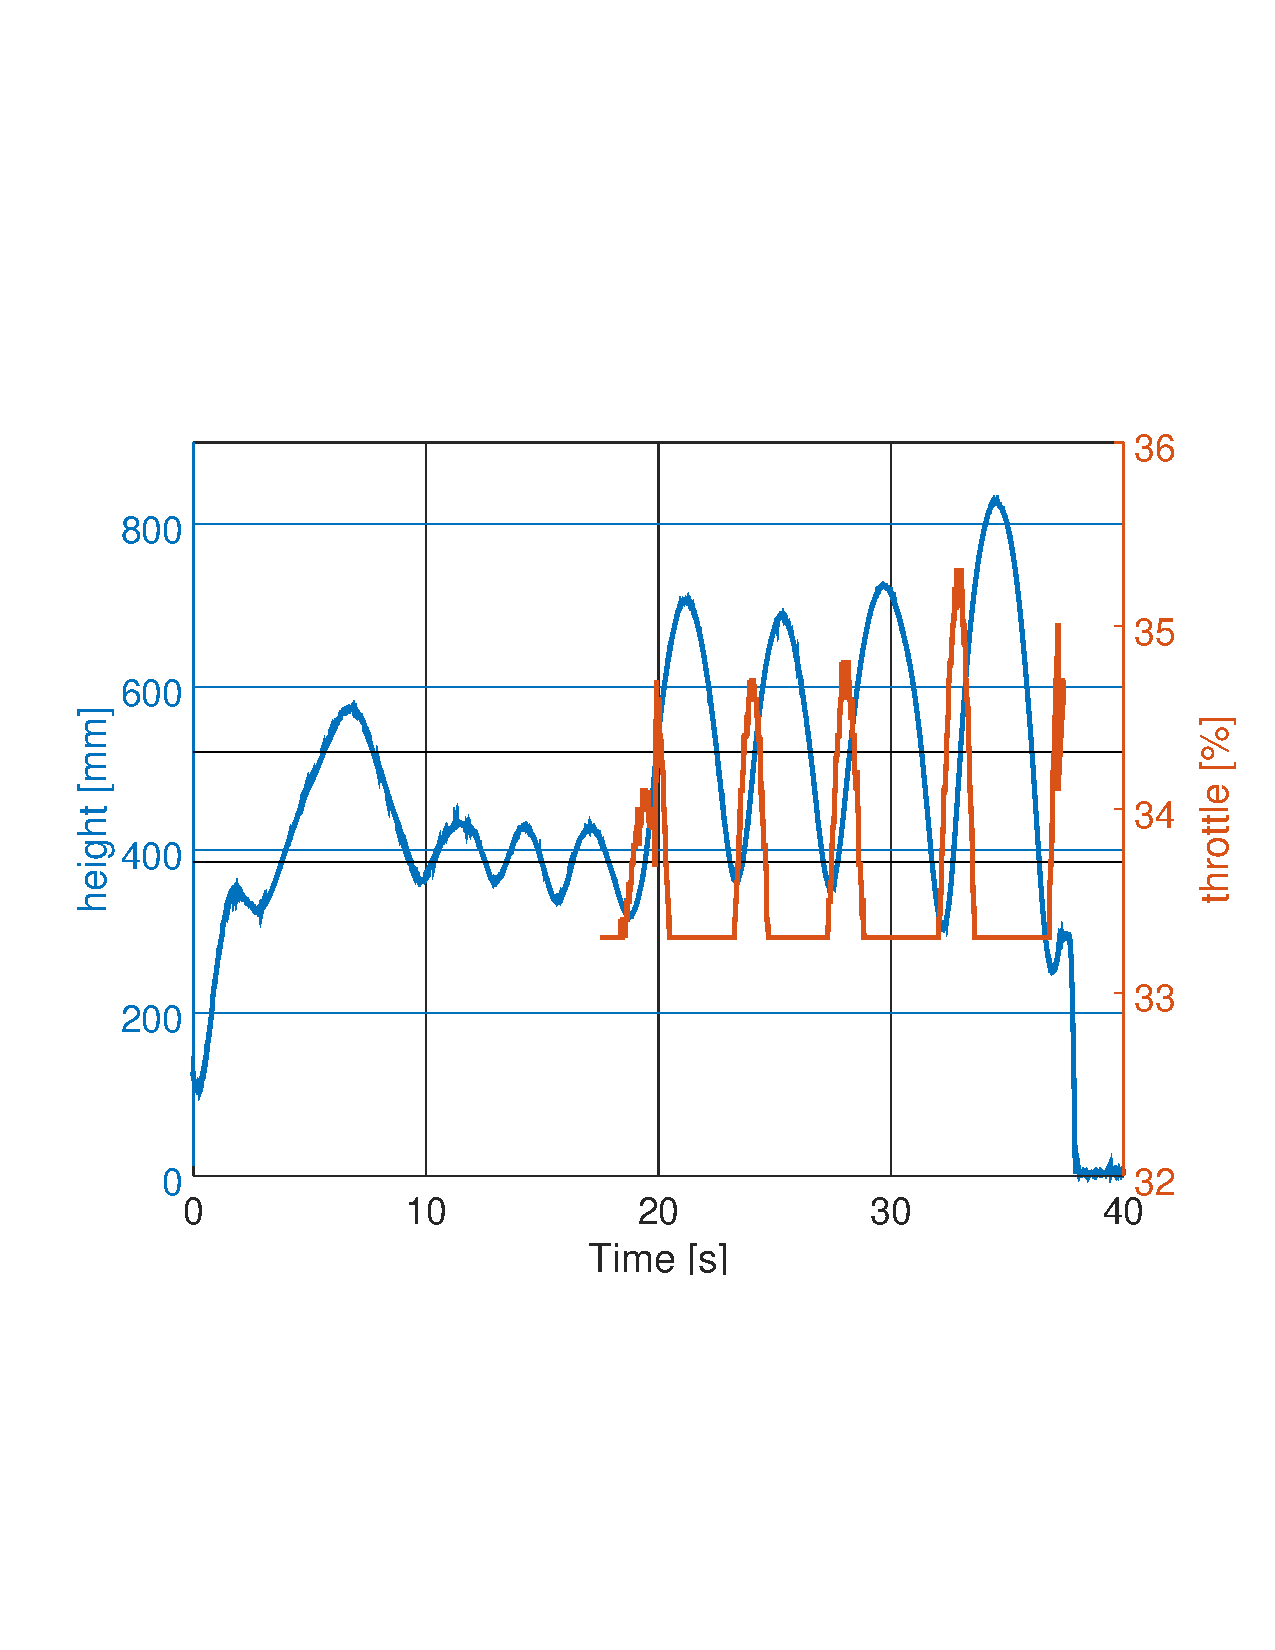
\includegraphics[width=0.6\textwidth, trim={0 7cm 0 7cm},clip]{figures/Appendix/final_test/kp0,1fix.pdf}
    \caption{Height graph K$_\text{p}$ = 0.1 with fixed saturation. Marker lines are at 385 and 520 mm}
    \label{fig:fourth_test_report}
\end{figure}

From the test result on figure \ref{fig:fourth_test_report} it can be seen that the system behaves as it should, when the set point is set 100 mm higher, the system regulates the throttle present to reach this height. The only problem with these results is the high overshoot is gives. and it is oscillating.

\subsection*{Conclusion for the final test}
As a conclusion for the final test, is that the system actually behaves as wanted. The only problem with the test is the high overshoot and oscillation. This problem might have to do with the addition of the K$_\text{p}$ value, this can have a influence on the overshoot and oscillation. So if the time had been to make the first tests again after figuring the fail in the code out, the oscillation and overshoot might have been avoided.

 The excessive oscillations and overshoot is due to the poor phase margin caused by the increased K$_\text{p}$ as can be seen on figure \ref{fig:bodeplot_final} Solutions to this will be discussed in the next chapter.

\begin{figure}[H]
    \centering
    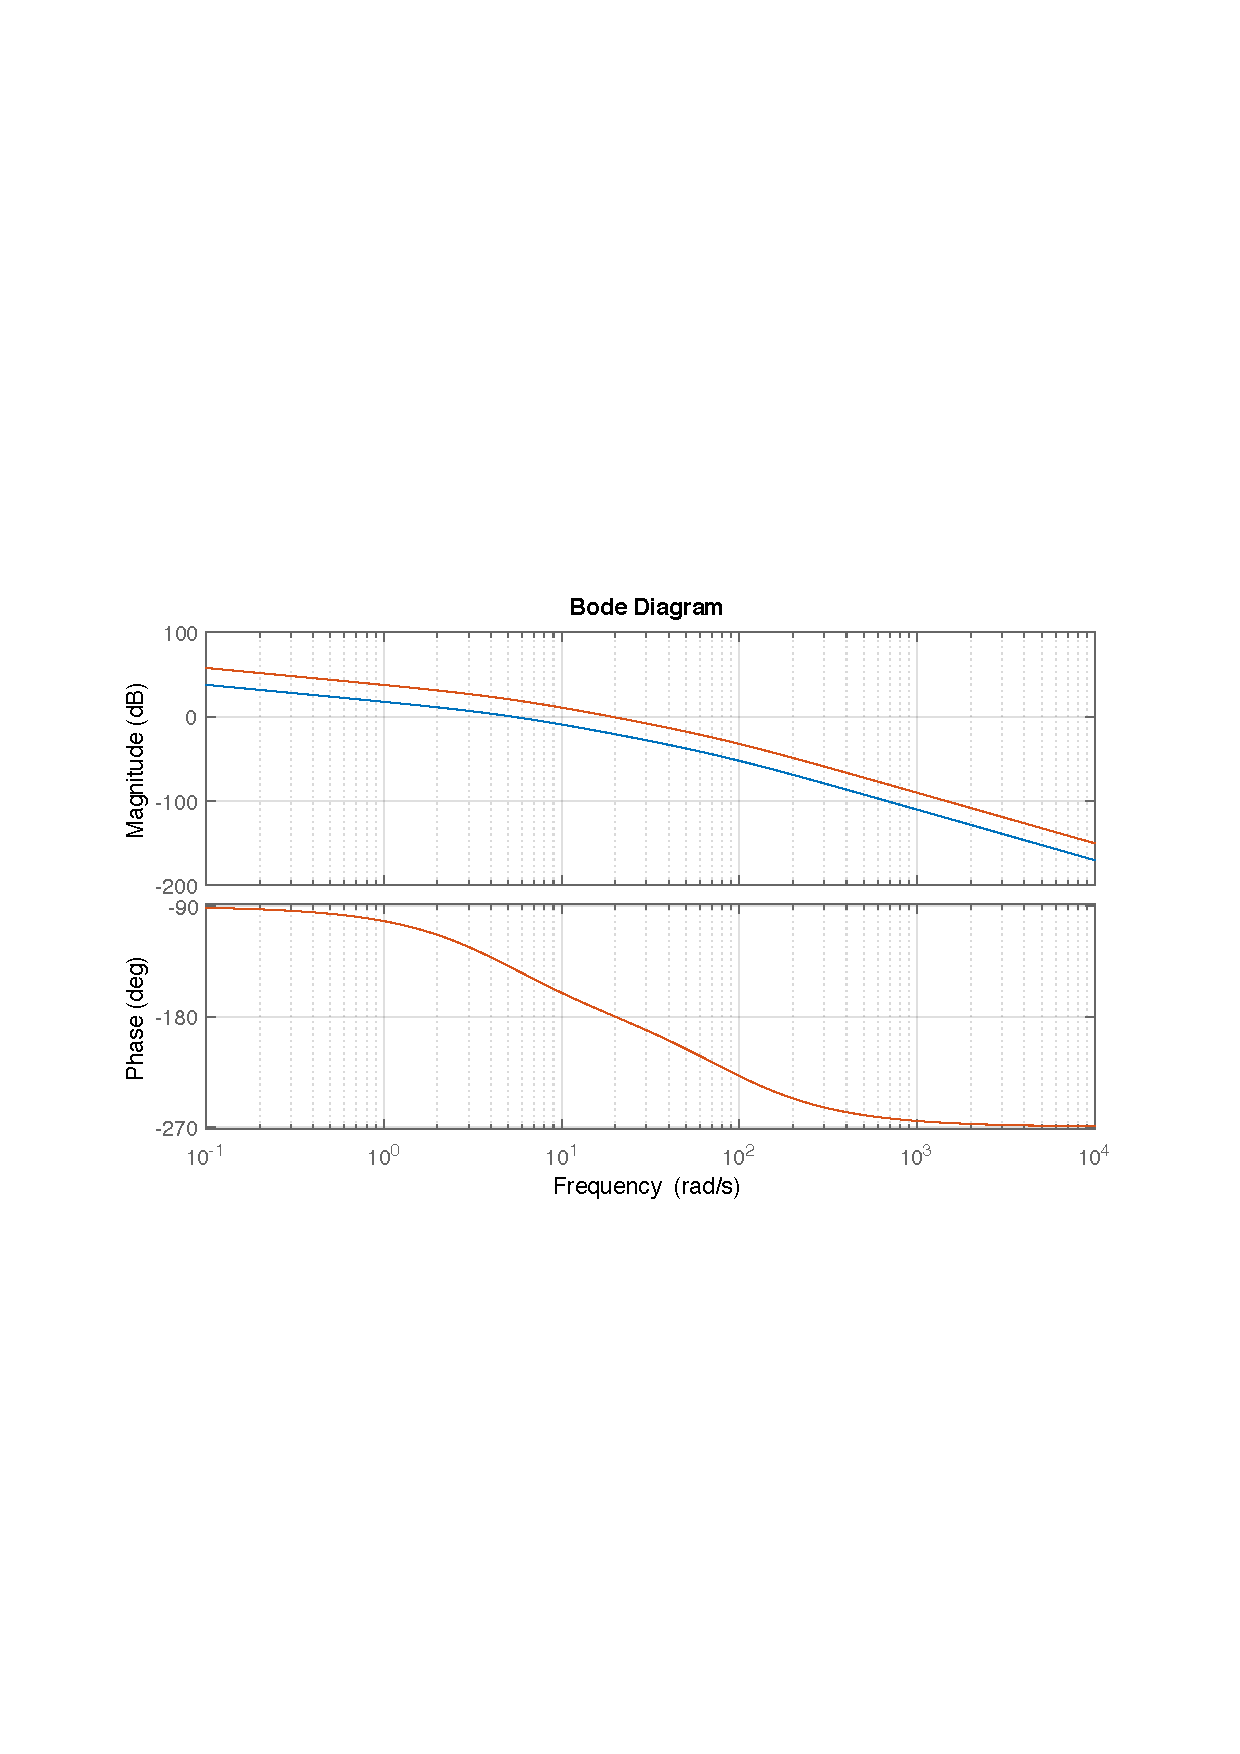
\includegraphics[width=\textwidth]{figures/Appendix/final_test/bodeplot_final.pdf}
    \caption{Bode plot for both the last tested K$_\text{p}$ and the calculated K$_\text{p}$.}
    \label{fig:bodeplot_final}
\end{figure}